% !TeX root = ../mde-presentation.tex

\subsection*{Plugins} \label{sec:plugins}

\begin{frame}{Plugins}
    \label{frm:plugins}
    Each research center has a different IT infrastructure and works with
    different frameworks. The aim of the model data explorer is to integrate
    these different systems into a user-friendly web-application. In order to
    be able to deploy the model data explorer at the different research
    centers, we aim for a modular structure where each component can be added
    or removed depending on the setup at the hosting institution.

    This modular structure is implemented via plugins. Each plugin is a python
    package containing a django app that can be added or removed from the
    configuration. We distinguish between three plugin categories:
    \hyperlink{frm:core}{core},
    \hyperlink{frm:framework-plugins}{framework} and
    \hyperlink{frm:service-plugins}{service} plugins.

    \vspace{2em}

    \begin{center}
        \begin{tabular}{p{0.4\textwidth}p{0.2\textwidth}p{0.3\textwidth}}
            \hyperlink{frm:framework-plugins}{\beamerbutton{\Large Framework plugins}} \\
            & \hyperlink{frm:core}{\beamerbutton{\Large Core}} \\
            & & \hyperlink{frm:service-plugins}{\beamerbutton{\Large Service plugins}}
        \end{tabular}
    \end{center}
\end{frame}

\begin{frame}{Framework plugins} \label{frm:framework-plugins}
    Framework plugins contain optionally but commonly used features for service
    plugins and are independent of the IT infrastructure.

    \begin{columns}[T]
        \begin{column}{0.45\textwidth}
            \begin{block}{mde-config}
                \begin{itemize}
                    \item defines a viewset-based structure where service
                        plugins can provide configuration interfaces for
                        individual datasets.
                    \item provides user configuration interfaces for the
                        \lstinline|mde-core| models.
                \end{itemize}
            \end{block}
            \begin{block}{mde-federation}
                \begin{itemize}
                    \item combines multiple MDE instances at different
                        institutions.
                    \item synchronizes datasets and data groups between
                        independant instances
                \end{itemize}
                \hyperlink{frm:federation}{\beamerbutton{Read more \ldots}}

            \end{block}
        \end{column}
        \begin{column}{0.45\textwidth}
            \begin{block}{mde-notifications}
                \begin{itemize}
                    \item implements the functionalities to send out
                        notifications to the users (e.g. for confirmations
                        required by dataset or data group owners)
                    \item provides an interface for the user for configuring
                        notifications
                \end{itemize}
            \end{block}

            \begin{block}{mde-oauth}
                \begin{itemize}
                    \item implements the possibility for the model data
                        explorer to serve as an OAuth or SAML Provider
                    \item gives attached services the possibility to
                        authenticate against the MDE and get
                        the users groups.
                \end{itemize}
            \end{block}
        \end{column}
    \end{columns}
\end{frame}

\begin{frame}{Service plugins} \label{frm:service-plugins}
    \begin{columns}
        \begin{column}{0.3\textwidth}
            Service plugins are based on the available IT infrastructure at a
            research institution. They connect a dataset of the
            \lstinline|mde-core| to an external service. This way, the MDE is
            configuring this external service.

            Service plugins should be independent of other service plugins (if
            possible) but they can depend on one of the
            \hyperlink{frm:framework-plugins}{framework plugins}.
        \end{column}
        \begin{column}{0.7\textwidth}
            \includegraphics[width=\textwidth, page=3]{figures/mde-service-plugins-basic.pdf}
        \end{column}
    \end{columns}
\end{frame}

\begin{frame}[t]{Planned service plugins}
    \begin{columns}[T]
        \begin{column}{0.45\textwidth}
            \only<1>{
                \begin{block}{mde-viewer}
                    A map-based viewer frontend for a dataset based on
                    ArcGIS4Javascript and angular. It displays all metadata and
                    services for an individual dataset. Services that are displayed
                    in this viewer are configured through the mde-esri,
                    mde-thredds, mde-analysis and mde-download plugins.
                \end{block}
                \begin{block}{mde-thredds}
                    This app creates catalog and configuration files for a
                    THREDDS-Server \citep{Caron1997} and restarts it when the
                    configuration changed.
                \end{block}
            }
            \only<2>{
                \begin{block}{mde-analysis}
                    The Analysis framework for the model data explorer.
                    Based upon the Data Analytics Software Framework
                    \citep[DASF, ][]{Eggert2022}
                    this plugin provides the framework to compute aggregated
                    analysis on datasets without the need to download the raw
                    data.
                \end{block}
            }
        \end{column}
        \begin{column}{0.45\textwidth}
            \only<1>{
                \begin{block}{mde-mams}
                    At Hereon, AWI and Geomar, we host instances of the
                    \textit{Media Assets Management System}, also called MAMS.
                    Through \lstinline|mde-mams|, users can request storage in
                    MAMS to upload netCDF files.
                    These workspaces are additionally mounted on the THREDDS-Server.
                \end{block}

                \begin{block}{mde-csw}
                    The \lstinline|mde-csw| plugin can combine multiple ISO-files
                    (e.g. generated via THREDDS) and provides an OGC-compliant CSW
                    endpoint via pycsw \citep{Kralidis2023}.
                \end{block}
            }
            \only<2>{
                \begin{block}{mde-download}
                    The download framework for the model data explorer. As
                    \lstinline|mde-analysis| based upon the DASF. This plugin
                    provides the framework to download subsets of the data.
                \end{block}
            }
        \end{column}
    \end{columns}

    \only<2>{
        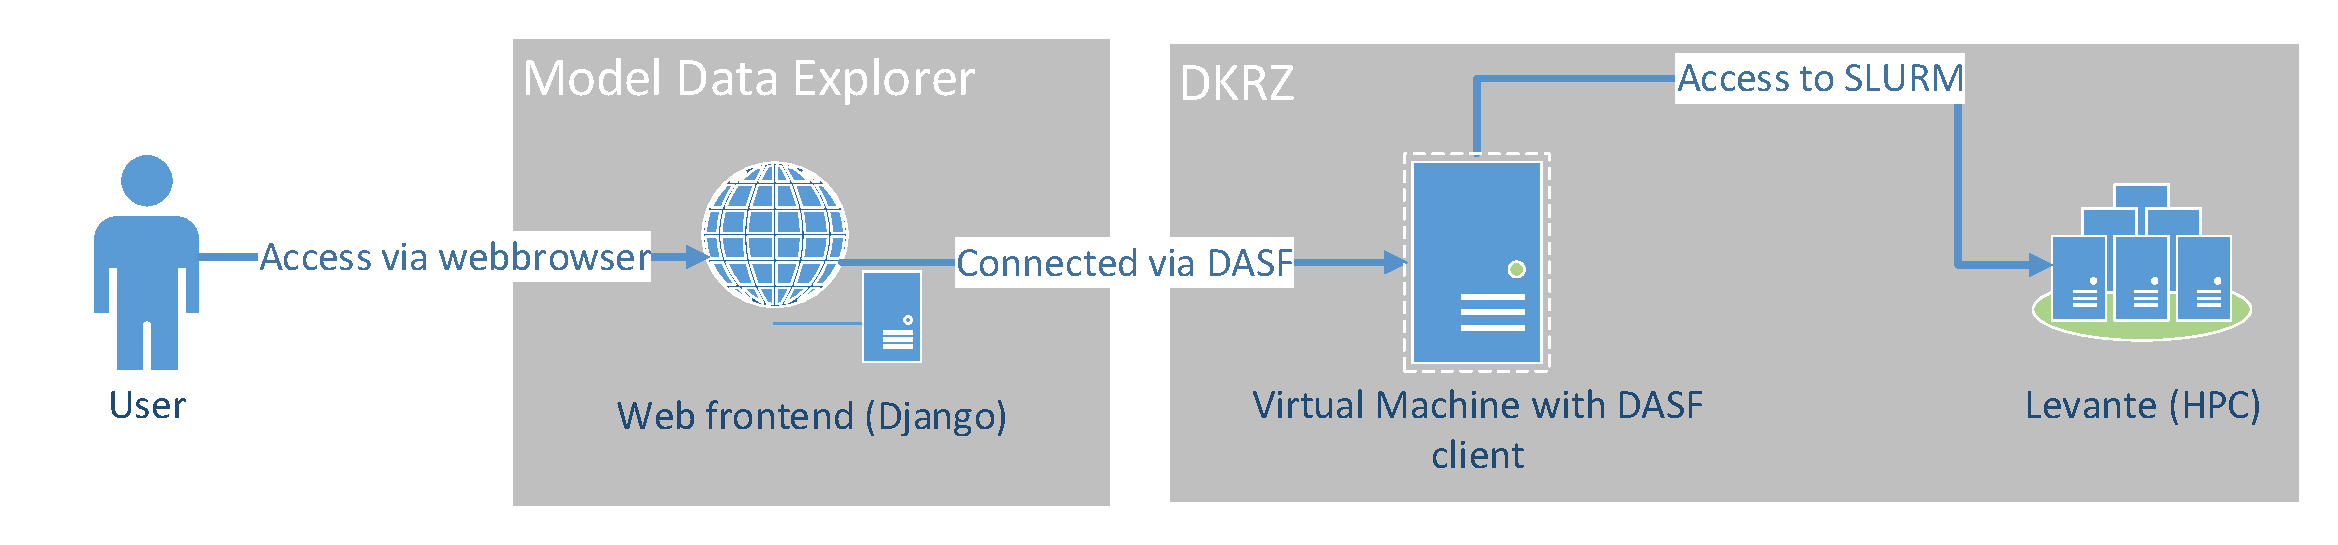
\includegraphics[width=\textwidth]{figures/dasf-schema.pdf}
    }

    \begin{textblock*}{\textwidth}(0.05\linewidth, 1.07\textheight)
		\slidebuttons
	\end{textblock*}

\end{frame}